\chapter{Designing a Scalable Qubit Architecture} \label{chapter:scalable_architecture}

In chapters \ref{chapter:processor_characterization} and \ref{chapter:grover_algorithm} we discussed the characterization and use of an elementary two-qubit quantum processor. With this processor, we demonstrated individual-qubit single-shot readout with up to \mbox{89 \%} readout contrast. We also implemented and characterized a universal $\sqrt{i\mathrm{SWAP}}$ two-qubit gate with \mbox{90 \%} gate fidelity and used it to run the Grover search algorithm, for which we obtained a single-run fidelity between $52\%$ and $67\%$, therefore demonstrating probabilistic quantum speed-up.

\smallskip

However, as we explain in this chapter, the approach to quantum computing that we presented cannot be scaled beyond a few qubits. Hence, in order to realize a larger-scale quantum computer it will be necessary to devise a new kind of scalable qubit architecture, where ``scalable'' means that the overhead for adding a qubit to a quantum processor does not require an exponential amount of physical or computational resources. In the literature, several proposals for scalable superconducting qubit architectures have been formulated, using e.g. a parametric coupling between qubits \citep{bertet_parametric_2006} or relying on the storage of quantum information in a separate entity, such as a superconducting resonator \citep{galiautdinov_resonatorzero-qubit_2012,mariantoni_implementing_2011}. In the following sections, we propose a different architecture, based on the recently introduced double-Transmon qubit \citep{gambetta_superconducting_2011,srinivasan_tunable_2011} and using a tunable qubit-qubit coupling scheme as well as a single-shot readout method for individual qubits. After giving a short overview of our proposed architecture, we show how we can implement a four-qubit processor with it. Furthermore, we discuss the possible limitations and shortcomings of the architecture. Finally, we put our work in context with other recent developments in the field of superconducting qubits and point out possible future research directions.

\section{Requirements} \label{section:scalable_architecture}

A scalable architecture for quantum computing should fulfill all of DiVincenzo's criteria as discussed in section \ref{section:divincenzo_criteria} and in addition not require an exponential experimental overhead in computational or physical resources for each qubit that is added to the quantum computer \citep{blume-kohout_climbing_2002}. Today, the two issues that are not addressed well by current qubit architectures (such as the quantum bus architecture used by many groups today \citep{dicarlo_demonstration_2009,wallraff_strong_2004}) concern the qubit-qubit coupling and the readout of individual qubits. The quantum bus architecture, for instance, has an ``always-ON''-type coupling scheme between the qubits, given by the Hamiltonian (\ref{eq:cqed_bus_coupling}). This scheme makes it hard to precisely control the coupling between individual qubits if a large number of them is present, since the effective coupling amplitude between any two qubits decreases $\propto 1/\Delta$ as a function of their detuning $\Delta$. Therefore, it becomes increasingly difficult and eventually impossible to deterministically switch on and off the coupling between individual qubits due to the limited available frequency space that can be allocated to each qubit (the so-called {\it frequency crowding}). Also, keeping track of all the involved phases and frequencies of the full coupled qubit register incurs a computational overhead that increases exponentially with the qubit number \citep{galiautdinov_resonatorzero-qubit_2012}. Using a direct capacitive coupling between individual qubits suffers from the same problem. Therefore, to be really scalable, a qubit architecture needs to have at least the following properties:

\begin{enumerate}
\item Well-defined qubits with long coherence times.
\item A single-shot, high-fidelity readout method for individual qubits.
\item High-fidelity single-qubit control.
\item Tunable and robust coupling between any two qubits.
\item Sub-exponential (ideally even sub-linear) scaling of resources when adding more qubits to the computer.
\end{enumerate}

As already said, the current CQED architectures fulfill most of these properties (to varying degrees) but fail to provide a tunable qubit-qubit coupling and a single-shot individual-qubit readout. In the following sections we discuss a proposal for an architecture that can potentially possess all of the above properties.

\section{Architecture Proposal}

Our proposed architecture follows the general CQED principles in that it uses Transmon qubits coupled to each other via a resonator acting as a quantum bus. However, instead of using a single Transmon to represent each logical qubit, we could use two of them that are capacitively coupled to each other and act therefore as a qubit ``molecule''. As shown by J. Gambetta {\it et. al.}, if we couple the two Transmons of such a molecule to the quantum bus with the same coupling constant, symmetry properties of the Hamiltonian of the molecule make it possible to fully decouple one of its eigenstates from the quantum bus \citep{gambetta_superconducting_2011}. This allows thus to remedy the problem of frequency crowding, since while the qubit is in this state (or in the ground state $\ket{0}$) no spurious coupling to other qubits will be present, regardless of the chosen qubit-qubit detuning. In the following section, we discuss the properties of this approach and the proposed qubit-qubit coupling scheme.

\subsection{The Double Transmon} \label{section:double_transmon}

\begin{figure}[ht!]
	\centering
	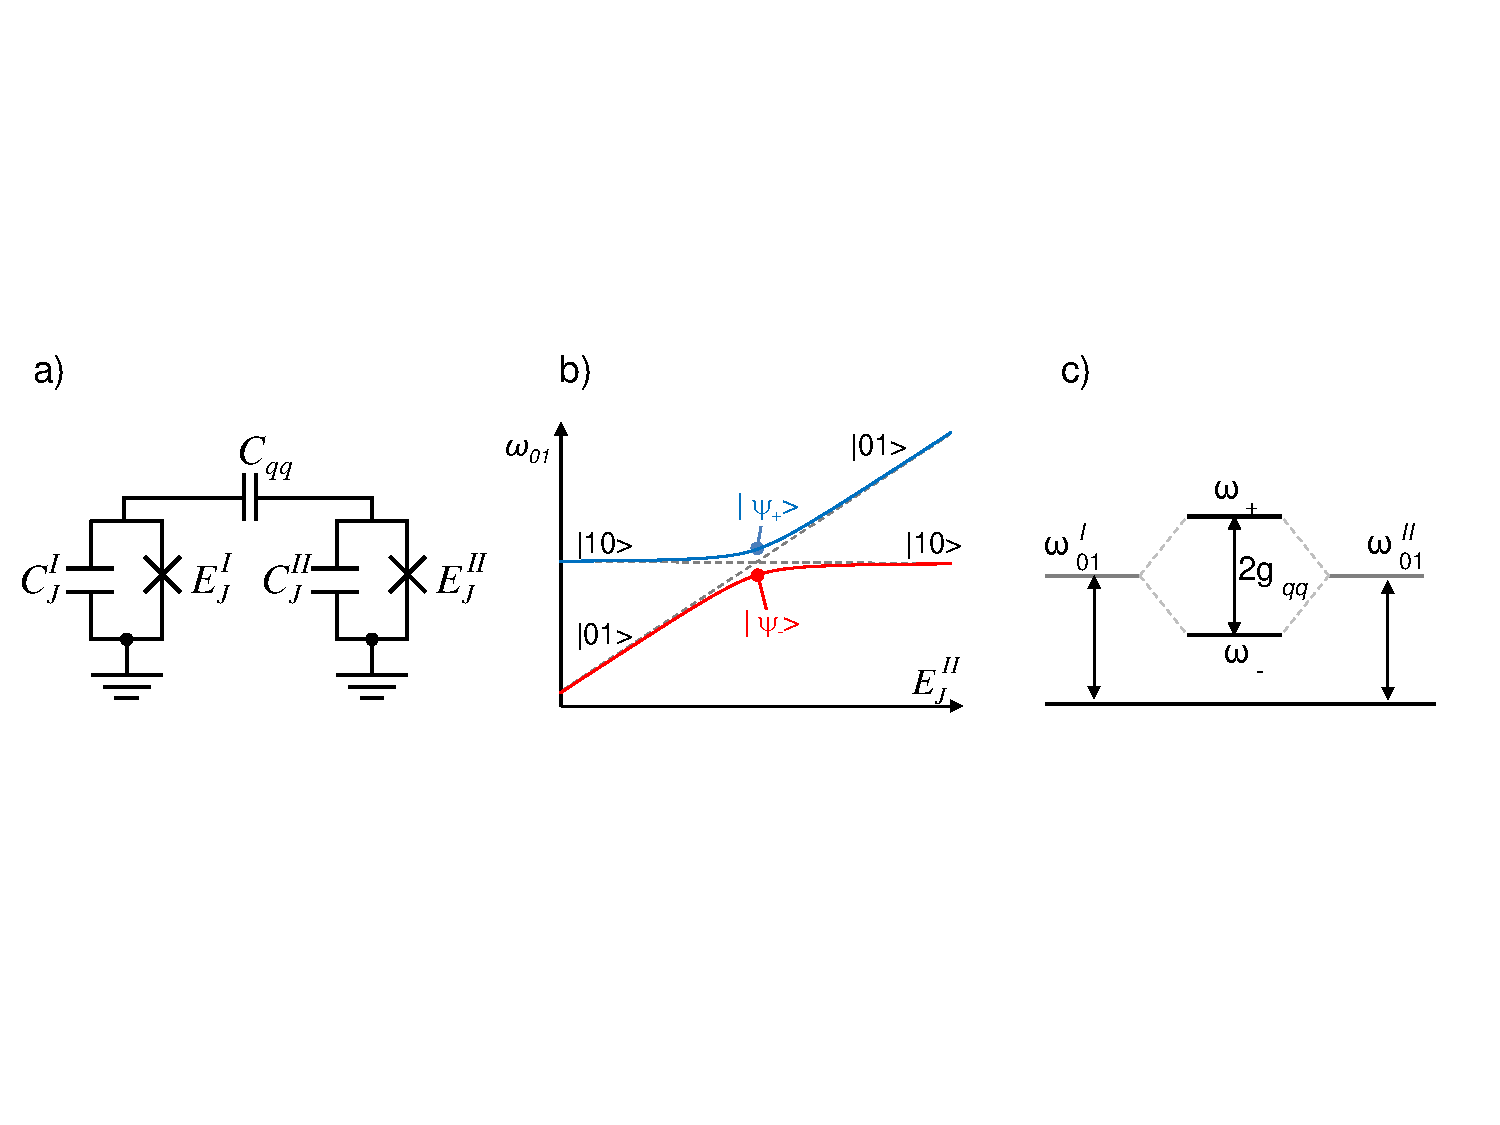
\includegraphics[width=\textwidth]{./material/figures/scalable-architecture/double_transmon_schematic}
	\caption{a) Schematic of the double Transmon qubit. b) Corresponding energy level diagram as a function of $E_J^{II}$. For $|\Delta|\gg g_{qq}$, the eigenstates are given as $\ket{00}$, $\ket{01}$, $\ket{10}$ and $\ket{11}$, whereas for $\Delta=0$, they are $\ket{00}$, $\ket{\psi_\pm}=(\ket{01}\pm\ket{10})/\sqrt{2}$ and $\ket{11}$, with eigen-energies $E_{00}=0$, $E_\pm = \hbar\omega_\pm = \hbar(\omega_{01}^{I,II}\pm g_{qq})$ and $E_{11}=\hbar(\omega_{01}^I+\omega_{01}^{II})$, as shown in c).}
	\label{fig:qubit_molecule_schematic}
\end{figure}

The Hamiltonian of the double Transmon (see fig. \ref{fig:qubit_molecule_schematic}) can be written as \citep{srinivasan_tunable_2011,gambetta_superconducting_2011}
%
\begin{eqnarray}
\hat{H}_{dt}       & = & \hat{H}_q+\hat{H}_{qq} \\
\hat{H}_{q}/\hbar  & = & \omega_{01}^I\hat{\sigma}_z^I+\omega_{01}^{II}\hat{\sigma}_z^{II} \\
\hat{H}_{qq}/\hbar & = & g_{qq}\left(\hat{\sigma}_+^I\hat{\sigma}_-^{II}+\hat{\sigma}_-^I\hat{\sigma}_+^{II}\right).
\end{eqnarray}
%
$\hat{H}_{dt}$ consists of the individual qubit Hamiltonians and the coupling Hamiltonian as given by eq. (\ref{eq:cqed_capacitive_coupling}). As before, we can rewrite $\hat{H}_{qq}$ in the two-qubit eigen basis $\ket{00}$, $\ket{01}$, $\ket{10}$, $\ket{11}$ of $\hat{H}_q$ as
%
\begin{equation}
\hat{H}_{qq}/\hbar = g_{qq}\left(\ket{10}\bra{01}+\ket{01}\bra{10}\right)
\end{equation}
%
When the qubit frequencies are on resonance such that $\Delta = \omega_{01}^I-\omega_{01}^{II}=0$, the eigenstates of $\hat{H}_{dt}$ are given as $\ket{00}$,$\ket{11}$, $\ket{\psi_+}=1/\sqrt{2}(\ket{01}+\ket{10})$ and $\ket{\psi_-}=1/\sqrt{2}(\ket{01}-\ket{10})$. Far off resonance, where $\Delta \gg g_{qq}$, the eigenstates will correspond to those of the uncoupled Hamiltonian $\hat{H}_{q}$. When coupling both Transmons to the cavity with the same coupling constant $g_{01}$ as given by eq. (\ref{eq:qubit_bus_coupling}) through the capacitance $C_{qb}$, we obtain a coupling Hamiltonian similar to eq. (\ref{eq:cqed_bus_coupling}):
%
\begin{equation}
\hat{H}_{qr}/\hbar = g_{01}\left(\hat{\sigma}_+^I\hat{a}+\hat{\sigma}_-^I\hat{a}^\dagger\right)+g_{01}\left(\hat{\sigma}_+^{II}\hat{a}+\hat{\sigma}_-^{II}\hat{a}^\dagger \right). \label{eq:double_transmon_resonator_coupling}
\end{equation}
%
Here, the Hamiltonian of the resonator is given by eq. (\ref{eq:lc_hamiltonian}). The coupling operator between the two qubits and the resonator contains the sums $\hat{\sigma}_+^{I+II}=\hat{\sigma}_+^I+\hat{\sigma}_+^{II}$ and $\hat{\sigma}_-^{I+II}=\hat{\sigma}_-^I+\hat{\sigma}_-^{II}$. Rewriting it in the eigen basis of $\hat{H}_{qq}$ at $\Delta=0$ yields the representation
%
\begin{equation}
\hat{H}_{qr} = \sqrt{2}g_{01}\left[\left(\ket{11}\bra{\psi_+}+\ket{\psi_+}\bra{00}\right)\hat{a}+\left(\ket{\psi_+}\bra{11}+\ket{00}\bra{\psi_+}\right)\hat{a}^\dagger\right].
\end{equation}
%
As can be seen, the qubit state $\ket{\psi_-}$ does not couple at all to the resonator, whereas the state $\ket{\psi_+}$ couples to it with an enhanced rate $\sqrt{2}g_{01}$. The states $\ket{01}=(\ket{\psi_+}+\ket{\psi_-})/\sqrt{2}$ and $\ket{10}=(\ket{\psi_+}-\ket{\psi_-})/\sqrt{2}$ couple to the resonator with the bare rate $g_{01}$. Thus, if we operate the double Transmon at $\Delta = 0$ and ``park'' the qubit in the state $\ket{\psi_-}$, we can effectively switch off the coupling to the resonator. To switch the coupling on again, we can perform an adiabatic transfer from the state $\ket{\psi_-}$ to the state $\ket{10}$ or $\ket{01}$ \citep{srinivasan_tunable_2011}. Alternatively, we can induce the transition $\ket{\psi_-}\to\ket{\psi_+}$ by using two single qubit pulses $X^I_\pi Y^{II}_\pi$, which however requires the possibility to drive each of the Transmons separately.

\smallskip

This coupling approach eliminates hence the frequency crowding problem and implements a fully controllable, on-demand qubit-qubit coupling scheme. In addition, parking the qubit in the state $\ket{\psi_-}$ reduces dephasing of the qubit state due to first-order flux noise, as explained in chapter \ref{chapter:processor_characterization}. 

%When taking into account the second Transmon level $\ket{2}$, the capacitive coupling induces additional coupling elements
%
%\begin{eqnarray}
%\hat{H}_{qq}'/\hbar g_{qq} &  = &  \left(\ket{10}\bra{01}+\ket{01}\bra{10}\right) \\
%& + & \sqrt{2}\left(\ket{11}\bra{02}+\ket{02}\bra{11}\right) \\
%& + & \sqrt{2}\left(\ket{11}\bra{20}+\ket{20}\ket{11}\right) \\
%& + & 2\left(\ket{21}\bra{12}+\ket{12}\bra{21}\right)
%\end{eqnarray}
%
%that we will ignore for now, but which become important when choosing the parameters of the double Transmon.

\section{Designing and Realizing A Four-Qubit Architecture}

\begin{SCfigure}[1.0][ht!]
	\centering
	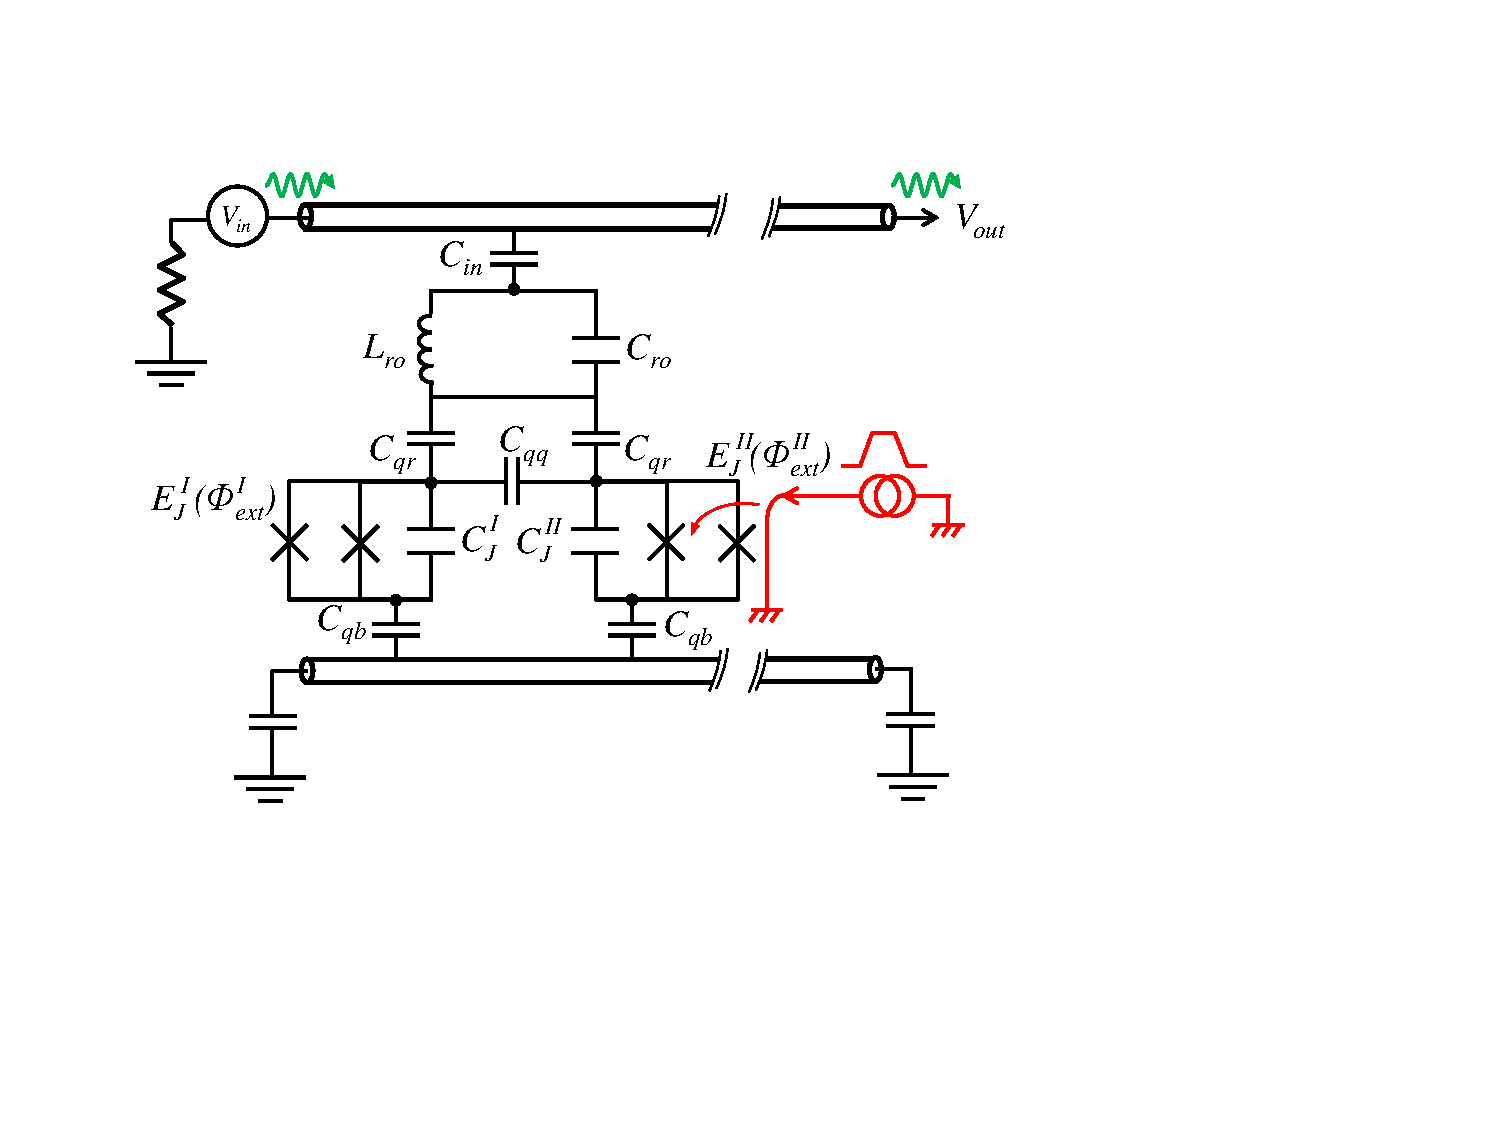
\includegraphics[width=0.6\textwidth]{./material/figures/scalable-architecture/double_transmon_architecture_schematic}
	\caption[]{Schematic of a qubit/readout unit cell of the proposed scalable architecture. Shown is a harmonic resonator capacitively coupled to an input transmission line and to two frequency-tunable Transmon qubits, which are in turn coupled to a coplanar waveguide $\lambda/2$ resonator that acts as a quantum bus to the other qubits. One of the two Transmons is equipped with a fast magnetic flux line. For sake of clarity we have omitted the capacitances of the LC resonator and the Transmon qubits to the ground node in the circuit schematic.}
	\label{fig:scalable_architecture_schematic}
\end{SCfigure}

The schematic of the proposed architecture is given in fig. \ref{fig:scalable_architecture_schematic}, showing a double Transmon capacitively coupled to a quantum bus (realized as a $\lambda/2$ transmission line resonator) and to a CJBA readout resonator, which is in turn capacitively coupled to an input transmission line. Each of the Transmons $I,II$ is realized as a split-CPB, thereby making it frequency-tunable through an external flux $\Phi_{ext}^{I,II}$. Since the coupling scheme as discussed in section \ref{section:double_transmon} requires only one of the two Transmons to be fast-frequency tunable, the design requires only one fast flux line per double Transmon. The flux of the other Transmon can be tuned to any desired bias point by using superconducting coils mounted above the chip, a technique which can be extended to a few qubits \citep{baur_realizing_2012}. The capacitive coupling of each of the two Transmons to the quantum bus and the readout resonator is identical, which is necessary in order to be able to cancel the interaction of the logical qubit with the resonator in the state $\ket{\psi_-}$, as discussed in section \ref{section:double_transmon}. 

\smallskip

As before, we can position the qubits at different, optimized frequencies for different processor operations. For qubit readout and driving, we can use a multiplexed input transmission line. In order to avoid crosstalk between individual readout resonators when driving them, we separate their resonance frequencies from each other by a small amount, typically \mbox{50 MHz}. The frequency of the quantum bus is chosen in function of the minimum qubit working frequencies such that the coupling of each qubit to the bus can be made sufficiently large to realize a two-qubit gate on a time scale that is small compared to the decoherence time of the qubits. 

\subsection{Processor Operation}

\begin{figure}[ht!]
	\centering
	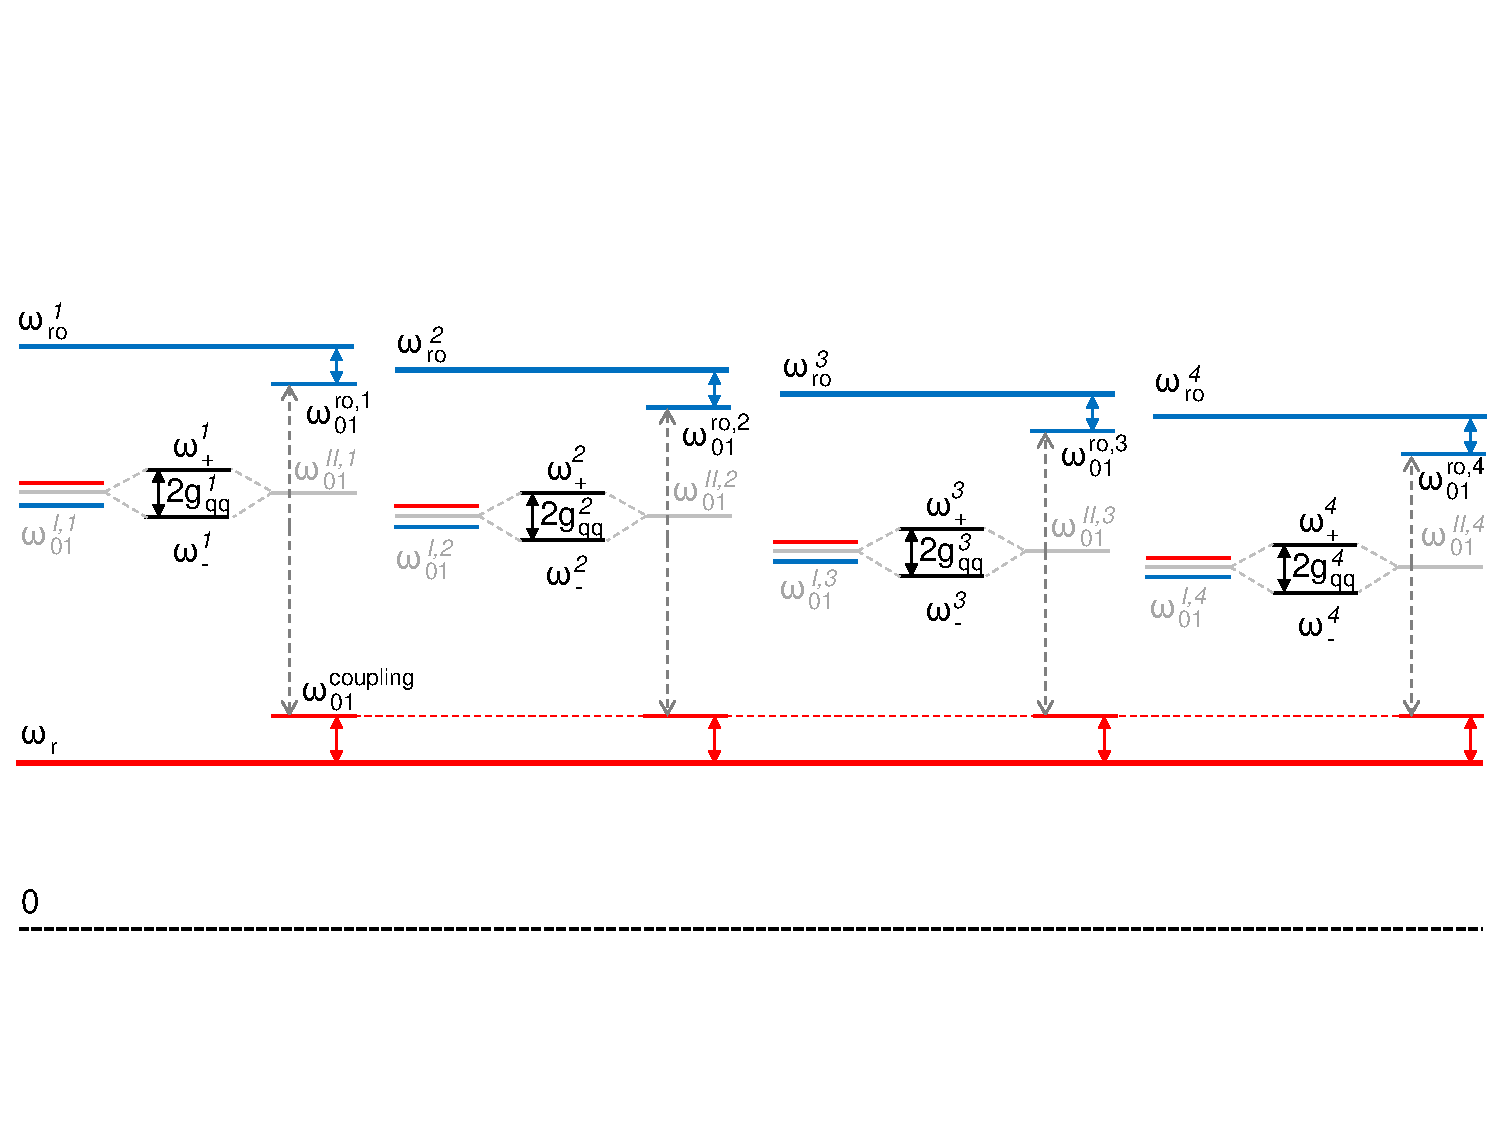
\includegraphics[width=\textwidth]{./material/figures/scalable-architecture/qubit_architecture_energy_levels}
	\caption[]{Operating frequencies of the proposed four-qubit processor, showing the frequencies of the quantum bus ($\omega_r$, red), the readout resonators ($\omega_{ro}$, blue) and the four double-Transmons qubits during parking (black), manipulation (red) or readout (blue). Grey bars indicate the frequencies of the uncoupled Transmon states.}
	\label{fig:scalable_architecture_energy_levels}
\end{figure}

Here we discuss the operation principles of the proposed quantum processor. In the following paragraphs, we refer to the individual qubit frequencies of the $i$-th double Transmon as $\omega_{01}^{I,i}$ and $\omega_{01}^{II,i}$ and define $\Delta_i = \omega_{01}^{I,i}-\omega_{01}^{II,i}$ as the detuning between them. In addition, we denote the logical qubit states of the i-th double Transmon as $\ket{x^i}$. 

\smallskip

As before, four basic processor operations need to be realized:

\begin{itemize}
\item Qubit parking (i.e. no operation)
\item Single-qubit gates
\item Two-qubit gates
\item Qubit readout
\end{itemize}

As for our two-qubit processor, for each of these operations we move the involved qubits to different frequencies, defining hence frequency bands for parking, qubit manipulation and qubit readout, as shown in fig. \ref{fig:scalable_architecture_energy_levels}. In the following paragraphs, we explain how we realize each of the operations mentioned above.

\subsubsection{Qubit Parking}

When not performing single-qubit or two-qubit operations, all qubits are ``parked'' by default. For this, each logical qubit $i$ is positioned at a common frequency $\omega_{01}^{I,i}=\omega_{01}^{II,i}=\omega_{01}^{\mathrm{park}}$, where its computational states are given as $\ket{00^i}$ and $\ket{\psi_-^i}$. The qubit is hence fully decoupled from the quantum bus and its readout resonator, eliminating the relaxation through the Purcell effect and the spurious coupling to other parked qubits of the processor. Qubit readout is also performed at the parking frequency (as explained below), hence this frequency should be chosen to provide an optimal readout contrast.

\subsubsection{Single-Qubit Gates}

To realize single-qubit gates, we perform an adiabatic passage from $\Delta_i = 0$ to $\Delta_i \gg g_{qq}^i$ by changing $\omega_{01}^{II,i}$, thereby performing a transfer $\ket{\psi_-^i}\to\ket{01^i}$. We can then drive the $\ket{00^i}\to\ket{01^i}$ transition of the qubit through the readout resonator or coupling bus and afterwards perform an adiabatic passage back to the parking position. Note that there will be a spurious coupling of the driven qubit to the $\ket{00}$ states of all parked qubits, which can be made small by choosing a sufficiently large detuning between the driving and parking frequencies, but which can nevertheless limit the scalability of this architecture for large numbers of qubits.

\subsubsection{Two-Qubit Gates}

To realize a two-qubit gate between the qubits $i$ and $j$, we adiabatically decrease the frequencies $\omega_{01}^{II,i}$ and $\omega_{01}^{II,j}$ to the point $\omega_{01}^{II,i}=\omega_{01}^{II,j}=\omega_{01}^{\mathrm{coupling}}$, performing an adiabatic transfer $\ket{\psi_-^i}\to\ket{01^i}$ and $\ket{\psi_-^j}\to\ket{01^j}$. At this frequency, there will be a resonant interaction between the logical qubits of the form $\hbar g_{qq}^{ij}(\ket{01^i,00^j}\bra{00^i,01^j}+\ket{00^i,01^j}\bra{01^i,00^j})$ with a coupling rate $g_{qq}^{ij}(\omega_{01}^\mathrm{coupling})=g_{01}^i g_{01}^j (\Delta_i^\mathrm{bus}+\Delta_j^\mathrm{bus})/2\Delta_i^{\mathrm{bus}}\Delta_j^\mathrm{bus}$, where $\Delta_i^\mathrm{bus}=|\omega_\mathrm{bus}-\omega_{01}^{II,i}|$ and $g_{01}^{i,j}$ are the qubit-resonator coupling constants of qubits $i$ and $j$. Please note that there will also be a spurious coupling of the same form to the $\ket{00}$ state of all other qubits $k$. This residual coupling can be made small by choosing a sufficiently large detuning $\omega_\mathrm{park}-\omega_\mathrm{coupling} \gg g_{qq}^{ik},g_{qq}^{jk}$, as explained in section \ref{section:qubit_qubit_coupling}.

\subsubsection{Qubit Readout}

To read out the state of qubit $i$, we perform an adiabatic passage to the state $\ket{10^i}$ by displacing $\omega_{01}^{II,i}$. This state can be read out using the dispersive interaction with the readout resonator. The parking frequency $\omega_{01}^\mathrm{park}$ at which the readout is performed should therefore be chosen such that the readout contrast is optimal.

\subsection{Design Parameters}

As before, we need to choose the maximum transition frequency $f_{01}^{max}$ and anharmonicity as well as the junction asymmetry for each qubit of the processor. The choice of these parameters has already been discussed in detail in chapter \ref{chapter:design} and will therefore not be repeated here. In addition, we need to choose the qubit-qubit coupling $g_{qq}$ and the qubit-resonator couplings $g_{01}^i$, for which we take into account the following criteria:

\smallskip

$g_{qq}$ should be large enough to be able to perform an adiabatic transition $\ket{\psi_-}\to\ket{01}$ in a time which is small compared to the relaxation and dephasing times of the qubit. We choose therefore a coupling $2g_{qq}/2\pi = 50\;\mathrm{MHz}$, which is large enough to be able to perform fast adiabatic transitions.

\smallskip

The qubit-resonator coupling $g_{01}^i$ should be sufficiently large to perform a two-qubit gate in a time small compared to the qubit decoherence time, yet not too large in order to avoid spurious coupling between the $\ket{01^i}$ state of the active qubits and the $\ket{00}$ state of the idling qubits during a gate operation. Taking the design of the two-qubit processor for reference, we choose $2g_{qq}^{ij}/2\pi = 10\;\mathrm{MHz}$ as the desired two-qubit coupling. For a qubit-resonator detuning $\Delta_i^\mathrm{bus}/2\pi=500\;\mathrm{MHz}$, the effective qubit-qubit coupling rate as given by eq. (\ref{eq:cqed_bus_coupling_rate}) then yields a required qubit-resonator coupling $g_{01}^i/2\pi\ge 71\;\mathrm{MHz}$. Assuming that we park the idling qubits at a detuning $\Delta_i^\mathrm{bus}/2\pi = 1\;\mathrm{GHz}$ to the bus while performing two-qubit gates, the chosen coupling corresponds to an acceptably low residual coupling amplitude of 1.5 \% between the active and idling qubits.

\smallskip

Finally, taking the design of the two-qubit processor as a reference, we choose a qubit-readout coupling (as generated by $C_{qr}$) of $g_{01}^{ro}/2\pi = 50\;\mathrm{MHz}$ and a qubit-readout resonator detuning $\Delta_i^\mathrm{ro}=1\;\mathrm{GHz}$ at the readout frequency. Using the same reference frequency band from 4-8 GHz as for the two-qubit processor, we choose the frequency of the quantum bus as $\omega_\mathrm{bus}/2\pi=4\;\mathrm{GHz}$ and the frequencies of the CJBA readouts as $\omega_{ro}^i/2\pi=7\;\mathrm{GHz}+i\cdot 60\;\mathrm{MHz}$, displacing the frequency between adjacent CJBAs by 60 MHz, which is sufficient to avoid crosstalk when driving the readout resonators. This yields a working frequency $\omega_{01}^\mathrm{coupling}=4.5\;\mathrm{GHz}$ for qubit-qubit coupling, a parking frequency $\omega_{01}^\mathrm{parking}=5.0\;\mathrm{GHz}$ and readout frequencies starting at $\omega_{01}^\mathrm{ro,I}=6.0\;\mathrm{GHz}$.

\subsection{Implementation}

\begin{figure}[ht!]
	\centering
	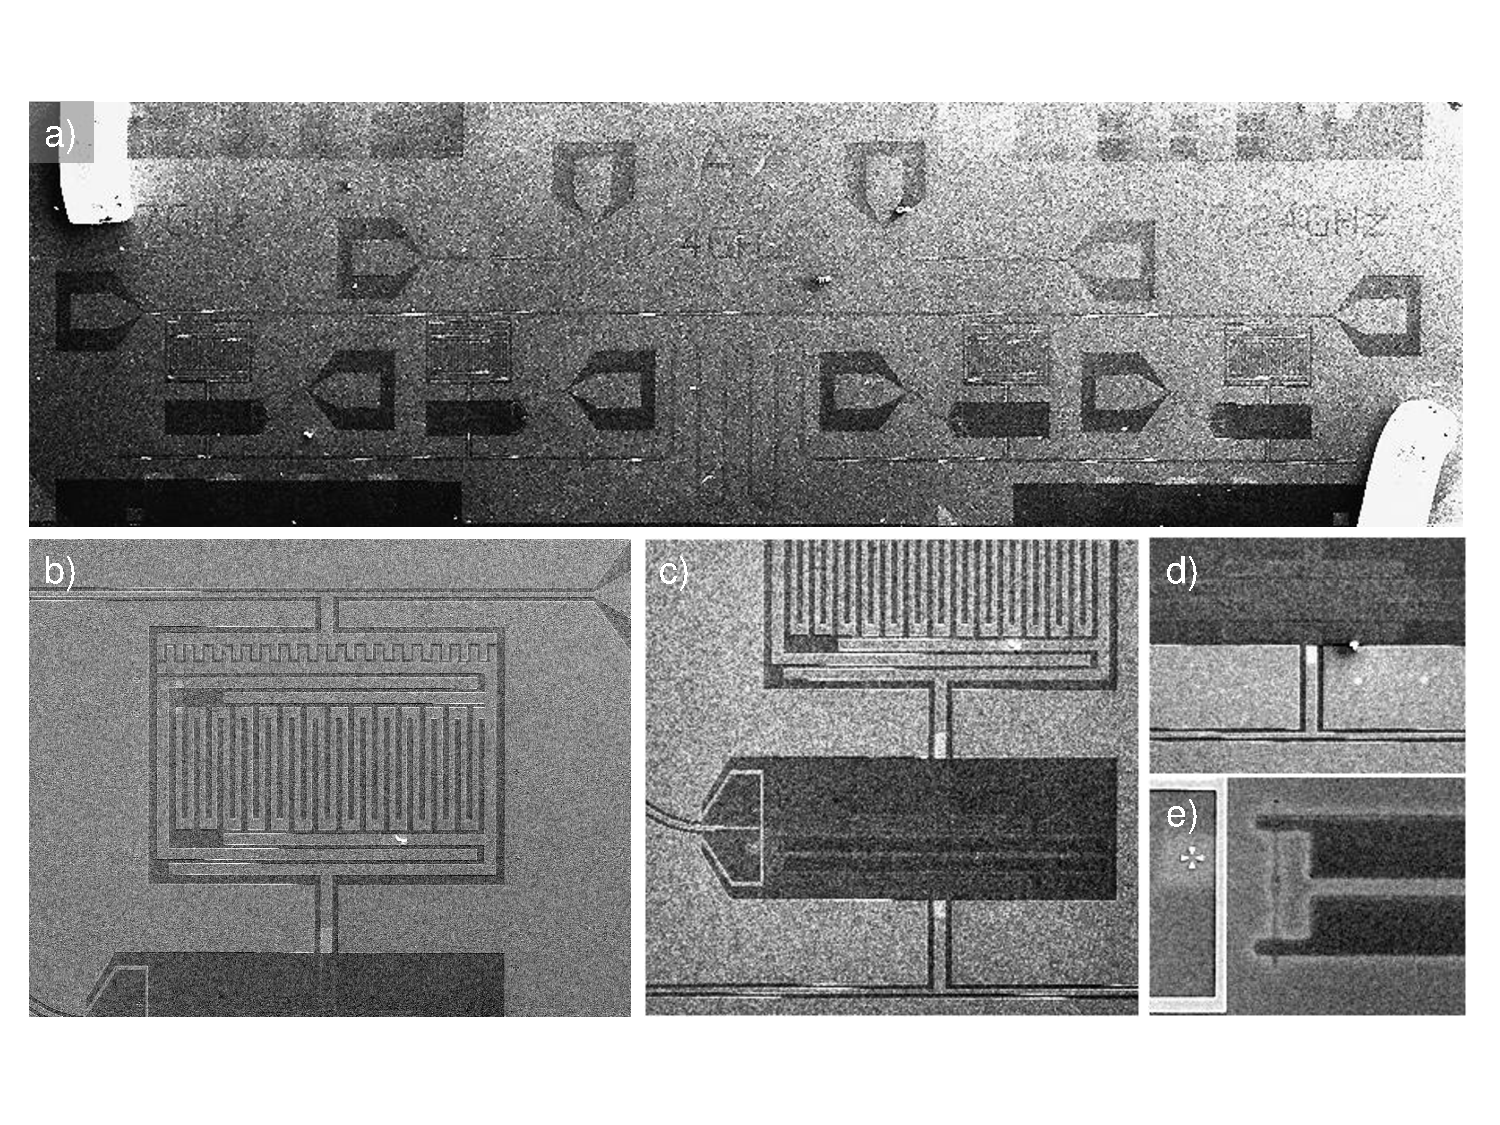
\includegraphics[width=\textwidth]{./material/figures/scalable-architecture/scalable_architecture_photos}
	\caption[]{Photos of the realized four-qubit chip. a) A stitched together image of the whole chip, showing the input transmission line, the readout resonators, qubit cells, fast flux lines and quantum bus. b) A detailed view of a single readout resonator, showing the CJBA realized in lumped elements and capacitively coupled to the input transmission line (above) as well as the qubit cell (below). c) A detailed view of a single Transmon qubit, which is capacitively coupled to its readout resonator and the quantum bus and inductively coupled to a fast flux line. d) The bus coupling capacitance of a single qubit. e) A detailed view of the qubit capacitance and SQUID as well as the adjacent fast flux line.}
	\label{fig:scalable_architecture_photos}
\end{figure}

Here we present the implementation of a ``predecessor'' of a full double-Transmon four-qubit architecture, where we use single Transmons instead to implement logical qubits, thereby simplifying fabrication and making it possible to test the readout and coupling elements of the proposed architecture without having to deal with the complexity of the double Transmons.

\smallskip

For the fabrication of the four qubit architecture, we use the same techniques as described in chapter \ref{chapter:design}. However, we change the design of the Transmon capacitance from an interdigitated to a parallel plate geometry, aiming to decrease the electric field strength inside the sample substrate, which was shown to be, to a large extent, responsible for intrinsic qubit dephasing and relaxation \citep{paik_observation_2011}. Furthermore, instead of using coplanar $\lambda/2$ resonators for the CJBA resonators, we implement them using lumped LC circuit elements, thereby significantly reducing their size. Again, all circuit components have been extensively modeled using microwave simulation software (SONNET) before fabrication. Fig. \ref{fig:scalable_architecture_photos} shows a series of SEM images of the realized single-Transmon four-qubit chip. First measurements carried out with this chip have been performed to test the qubit manipulation and readout, and will be discussed in the thesis of V. Schmitt. As an example, fig. \ref{fig:jba_multiplexed_spectroscopy_main} shows a microwave transmission measurement of the four multiplexed JBA readouts on the chip.

\begin{SCfigure}[1.0][ht!]
	\centering
	\includegraphics[width=8.8cm]{"./data/scalable architecture/jba spectroscopy/spectro"}
	\caption[Measured $|S_{12}|$ transmission coefficient for the input transmission line of our four-qubit chip]{Measured $|S_{12}|$ transmission coefficient of drive and readout line of our four-qubit chip, with the four qubits far detuned from the resonators. Clearly visible are the resonances of the four CJBA resonators and their bifurcation at nominal input powers between -42dB and -40 dB.}
	\label{fig:jba_multiplexed_spectroscopy_main}
\end{SCfigure}

\subsection{Scalability of the Proposed Architecture}

The proposed qubit architecture solves the problem of individual-qubit single shot readout and tunable qubit-qubit coupling for a single register of logical qubits coupled to a quantum bus. The architecture requires $n+1$ fast signal lines and $n$ DC bias lines for $n$ qubits, hence being scalable with a linear increase in resources. However, the size of the qubit-resonator coupling capacitances limits the number of qubits that can be coupled to a single quantum bus, since placing the capacitances too close to each other will induce spurious qubit-qubit coupling. Furthermore, the spurious couplings of the form $\ket{00^i,01^j}\ket{01^i,00^j}+\ket{01^i,00^j}\bra{00^i,01^j}$, which are always present during single- and two-qubit gates, can induce further unitary errors. Our proposed architecture is thus not intrinsically scalable beyond a few tens of qubits. In order to scale further, it would therefore be necessary to use several independent registers of qubits, each connected to a separate quantum bus and coupled together by using ``shuttle'' qubits. These shuttle qubits would be coupled to two or more quantum buses and act solely as tunable couplers between different registers, as proposed e.g. by \citep{divincenzo_physical_2000,palacios-laloy_superconducting_2010}.

\section{Conclusions}

We propose a four-qubit architecture based on double-Transmon qubits that can potentially alleviate current problems of superconducting qubit architectures such as frequency crowding and could allow the scaling up of superconducting quantum processors to a few tens of qubits. Viewing the recent experimental advances in Transmon relaxation and dephasing times \citep{paik_observation_2011} that allow for a large number of quantum gates during the qubit's coherence time, the dominant roadblock on the way to scalable superconducting quantum computing seems today to be the realization of a tunable coupling scheme for a large number of qubits. Besides the possible approach presented here, different proposals have been made for solving this issue by relying e.g. on isolating logical qubits by storing their quantum information in resonators \citep{galiautdinov_resonatorzero-qubit_2012,mariantoni_implementing_2011} or quantum memories based e.g. on electronic or nuclear spins \citep{zhu_coherent_2011,kubo_storage_2012,kubo_hybrid_2011}.